\section{Introduction}
\paragraph{Image-to-image translation}
Image-to-image translation has drawn a lot of attention recently, which aims to apply an image in one domain to generate a corresponding image in another, reserving shared concepts, objects or scenes in these two images.  
 
Generating a corresponding image from an input image can be reformulated as a conditional image generation problem which is conditioned on the input image. Previous works about conditional image generation problem focused on generating images from discrete labels~\cite{CGAN}, texts~\cite{reed1, reed2} and images.
\cite{pix2pix} firstly introduced the concept of image-to-image translation and trained a framework by paired images to handle multiply applications, such as labels to street scene, day to night, edge to photo and etc., only switching the training datasets.
%
\cite{a,b,c,d} extend the translation with difficultly and expensively achieved paired image datasets to unpaired image datasets, and they hugely widened the application to cover the scene where the desired outputs are highly complex or not even well-defined.

However, the previous works share a common shortage that the generated images always reserve the edge layout of the input images. 




\section{Related work}
\subsection{Sketch}
Sketches has been well studied in past years. \cite{HowSketch} released a large sketch dataset with 20K sketches in 250 categories and proposed a sketch classification method based on a bag-of-feature sketch representation and multi-class support vector machines. 
%
\cite{SketchANet} achieved a sketch classification performance surpassing that of humans by developing two data augmentation strategies to significantly increase the volume and diversity of sketches and exploring different network ensemble fusion strategies to improve the classification performances.
\cite{sketch3dshape} introduced a sketch-based 3D shape retrieval method that trained two siamese convolutional neural networks to learning the views for 3D shape and the sketches.
Unlike works prior to it which have retrieved images in the same category of the query sketch, \cite{sketchmethatshoe} addressed a fine-grained sketch-based image retrieval problem that required instance-level retrieval of images. They trained a siamese networks with a newly collected dataset of sketch-photo pairs and applied staged pre-training and fine-tuning.

\subsection{Conditional Generative Adversarial Networks}
Our work is based on generative adversarial networks (GANs)~\cite{GAN} in conditional setting. In a typical GAN, a generative net and a 

Previous works have explored GANs generating images in the condition of discrete labels~\cite{CGAN}, text~\cite{reed1, reed2} and images. 
Conditional GANs were firstly introduced by \cite{CGAN} who treated the conditional generation problem as the inverse processing of image classification and used discrete labels as condition to generate images.
%
\cite{Dosovitskiy} trained convolutional networks to generate images of objects given object style, viewpoint and color. With the experiments of interpolating viewpoints, they showed that networks learn a meaningful representation of 3D models. 
%
\cite{reed1, reed2} generated photo-realistic images conditioned on text descriptions.

\subsection{Image-to-image translation with GANs}
Given an image in one domain, image-to-image translation methods generate a corresponding image in another. These two images are possible representations of the same scene. Image-to-image translation with GANs is a special case of conditional GANs where images are applied to be conditions. 
%

\cite{pix2pix} firstly introduced the concept of image-to-image translation, who treated one image in a paired image dataset as conditioned input and generate its corresponding image. Unlike works prior to it which dealt with only one application, \cite{pix2pix} are able to handle multiple applications in one frame work only switching training datasets. They applied skip connections between mirrored layers in the generator to make sure low-level information pass through its encoder-decoder architecture and used dropout in stead of random vector to provide stochasticity in the networks.
%
\cite{unit} studied on unpaired image-to-image translation by training a two-branch GAN. Each branch is composed with a encoder, a generator and a discriminator. With the idea that high-level representation of a pair of corresponding images in two domains should be the same, high-level layers share weights between two branches in encoders, generators and discriminators. 
%

CycleGAN~\cite{CycleGAN}, DiscoGAN~\cite{DiscoGAN} and DualGAN~\cite{DualGAN} developed similar architectures to translate unpaired images which contain, for each, two generators and two discriminators. These methods learn two mappings in an adversarial training process such that an input image in one domain is mapped to a generated image in another, and then the generated image is mapped to a reconstructed image which is closed to the input image in some measures. These methods shared the same idea that since the generated image is able to reconstruct the input image, it should contain the content of the input image.

\section{Exploration}
\subsection{CycleGAN}
\subsubsection{Details}
\paragraph{Residual blocks}
In spired by \cite{Johnson et. al.}, in the bottleneck layers, residual blocks~\cite{ResNets} are added to transfer features of input image to features of generated image. 
\paragraph{Instance normalization}
Instance normalization is also unknown as contrast normalization. CycleGANs swap batch normalization with instance normalization in both training and testing time since we want to keep the content instead of style and contract is clearly not a part of content in the image.
\paragraph{Generated image pool}
CycleGANs discard both random vectors and dropout which introduce stochasticity in the training procedure and use the historical generated images to update the discriminators by maintaining a generated image pool with size of 50. The pool is filled with first generated 50 images and updated by replacing one of randomly selected images in it with the newly generated image.
%
\begin{figure}
	\label{cyclegan_reported_results}
	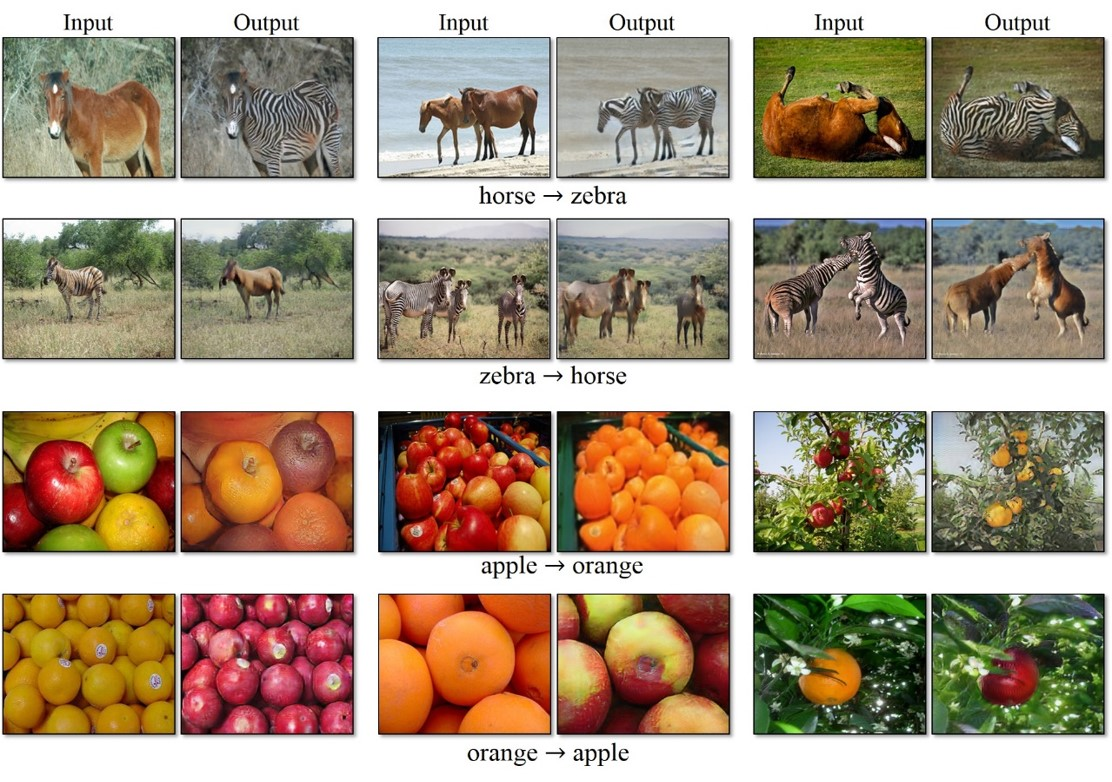
\includegraphics[width=0.5\textwidth]{figures/cyclegan/reported_results.jpg}
	\caption{Reported results of CycleGAN.}
\end{figure}
%
\begin{figure}
	\label{cyclegan_sketch2photo_apple_200epochs_torch}
	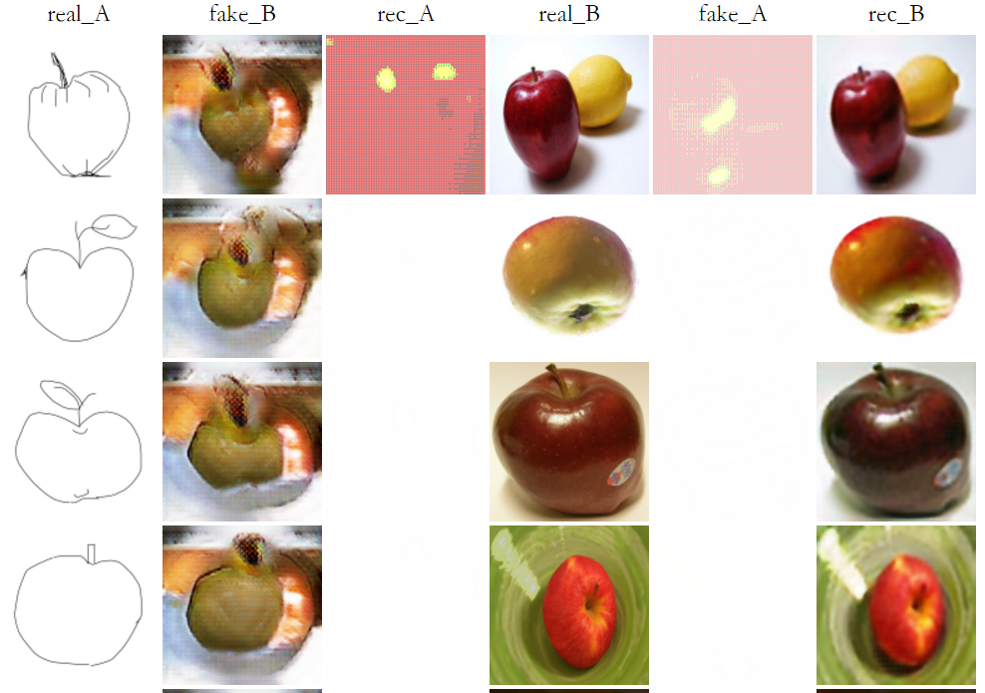
\includegraphics[width=0.5\textwidth]{figures/cyclegan/sketch2photo_apple_200epochs_torch.png}
	\caption{Results of CycleGAN on sketch-to-photo dataset of apples. <TODO> description}
\end{figure}
%
\begin{figure}
	\label{cyclegan_sketch2photo_airplane_200epochs_torch}
	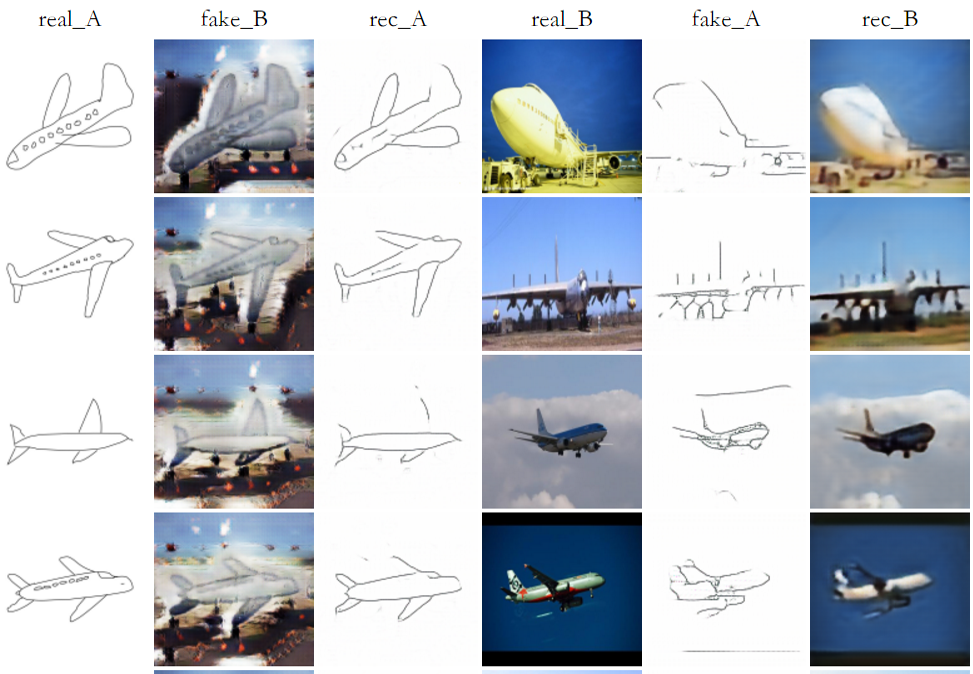
\includegraphics[width=0.5\textwidth]{figures/cyclegan/sketch2photo_airplane_200epochs_torch.png}
	\caption{Results of CycleGAN on sketch-to-photo dataset of airplanes. <TODO> description}
\end{figure}
%
%
\subsubsection{Results of sketch-to-photo translation}
Figure~\ref{fig:cyclegan_reported_results} shows the reported results of CycleGAN. Notice that, taking horse-to-zebra as example, only the horse in the input image rather than the whole image is translated into black and white, which is different from style transfer where the styles of both the object and background are transfered. Also, the green grass in the background is translated into brown, the color of the environments zebras live in.

However, when we train CycleGAN with the sketch-to-photo dataset ("real\_A" and "real\_B" in figure~\ref{fig:cyclegan_sketch2photo_apple_200epochs_torch} and ~\ref{fig:cyclegan_sketch2photo_airplane_200epochs_torch}, results are not as good as the other. As illustrated, both models suffer from severe issue of mode collapse, a common but unsolved problem of training GANs that input images of different modes are mapped to images of the same mode in corresponding domain. Also, the edges of the input images are preserved in the generated images. This is acceptable in some application like horse-to-zebra or apple-to-orange, since the contours of the the input objects and output objects are similar to each other. However, when it comes to the sketch-to-photo, the preserving of edges is unexpected since objects in generated photos with free-hand style contours are not visually real.

Another 
